\subsection{Regression mit ARMA-Fehlern}
\begin{frame}{Regression mit ARMA-Fehlern}
	\underline{Gegeben}: 
	\begin{itemize}
		\item Beobachtungen $(y_1,...,y_T)$ der Zeitreihe $(y_t)_t$
		\item Beobachtungen $(x_1^{(i)},...,x_T^{(i)})$ der Zeitreihen $(x_t^{(i)})_t$ für $i=1,...,k$
	\end{itemize}
	\textbf{Modellgleichung: Regression mit ARMA(p, q)-Fehlern} \cite{forecasting}\\
	\begin{align*}
		y_t &= c + \sum_{j=1}^{k}\beta_j x_t^{(j)} + \eta_t \text{ mit} \\
		\eta_t &= \underbrace{\sum_{k=1}^{p}\phi_p\eta_{t-p}}_{\text{vergangene Fehler: LM}} + \underbrace{\sum_{l=1}^{q}\theta_l\epsilon_{t-q}}_{\text{vergangene Fehler: ARMA}} + \epsilon_{t}
	\end{align*}
\end{frame}

\begin{frame}{Regression mit ARMA-Fehlern}
	Vorarbeit:
	\begin{itemize}
		\item Überprüfung Autokorrelation der Zielvariablen (Acf, pAcf)
		\item Standardisierung Train, Skalierung Test
	\end{itemize}
	Überprüfung der Voraussetzungen:
	\begin{itemize}
		\item Stationarität aller Variablen (Augmented Dickey-Fuller Test)
		\item keine Multikollinearität vorhanden (VIF)
		\item Normalverteilung der Residuen (Scatterplot, Histogramm, QQ-Plot)
	\end{itemize}
\end{frame}

\begin{frame}{Bestimmung des Grids für die AR-Ordnung - Uplink}
		\begin{figure}
			%\centering
			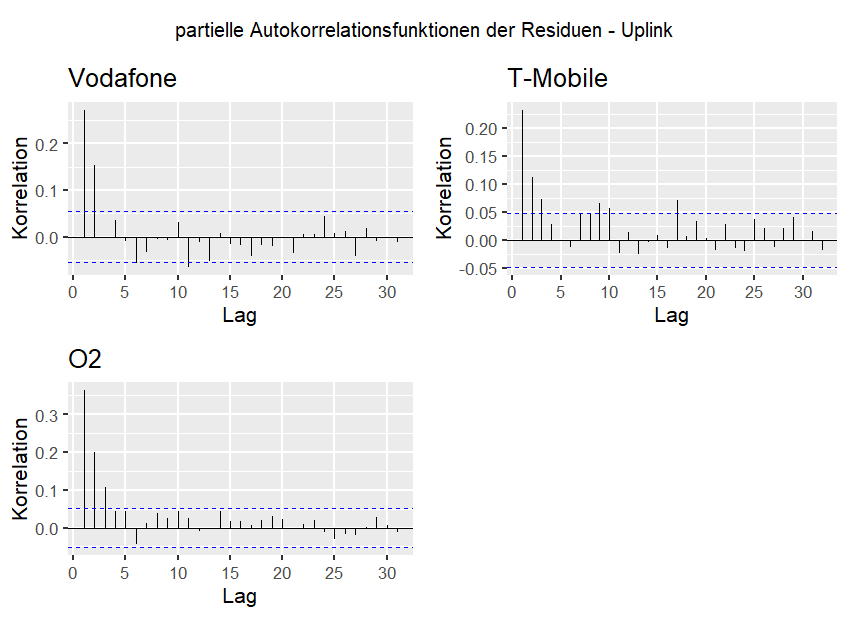
\includegraphics[scale=0.42]{plots/arima/uplink/res_pacf}\\
			\label{res_pacf_ul}
		\end{figure}
\end{frame}

\begin{frame}{Bestimmung des Grids für die MA-Ordnung - Uplink}
		\begin{figure}
			%\centering
			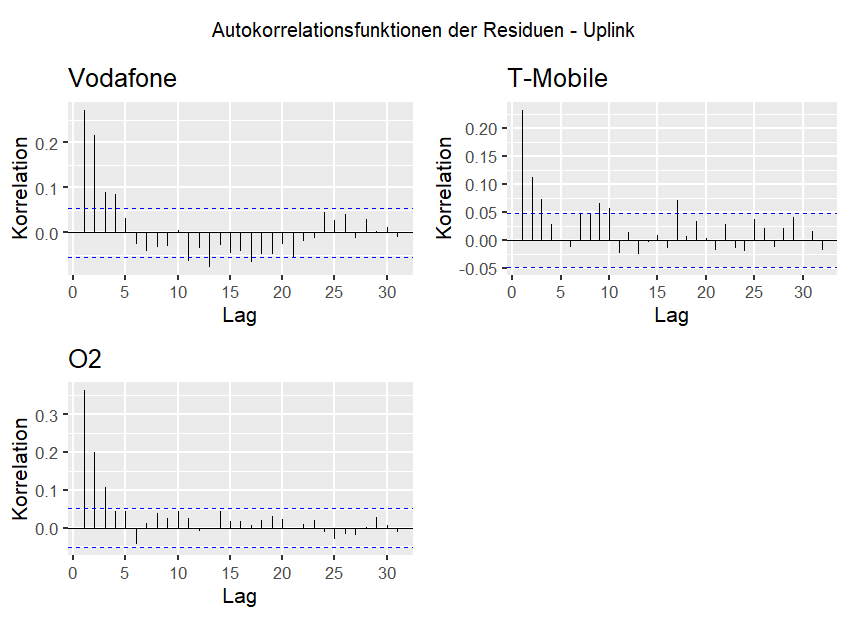
\includegraphics[scale=0.42]{plots/arima/uplink/res_acf}\\
			\label{res_acf_ul}
		\end{figure}
\end{frame}

\begin{frame}{Regression mit ARMA-Fehlern: Ergebnisse (Uplink)}
	\begin{figure}
		\centering
		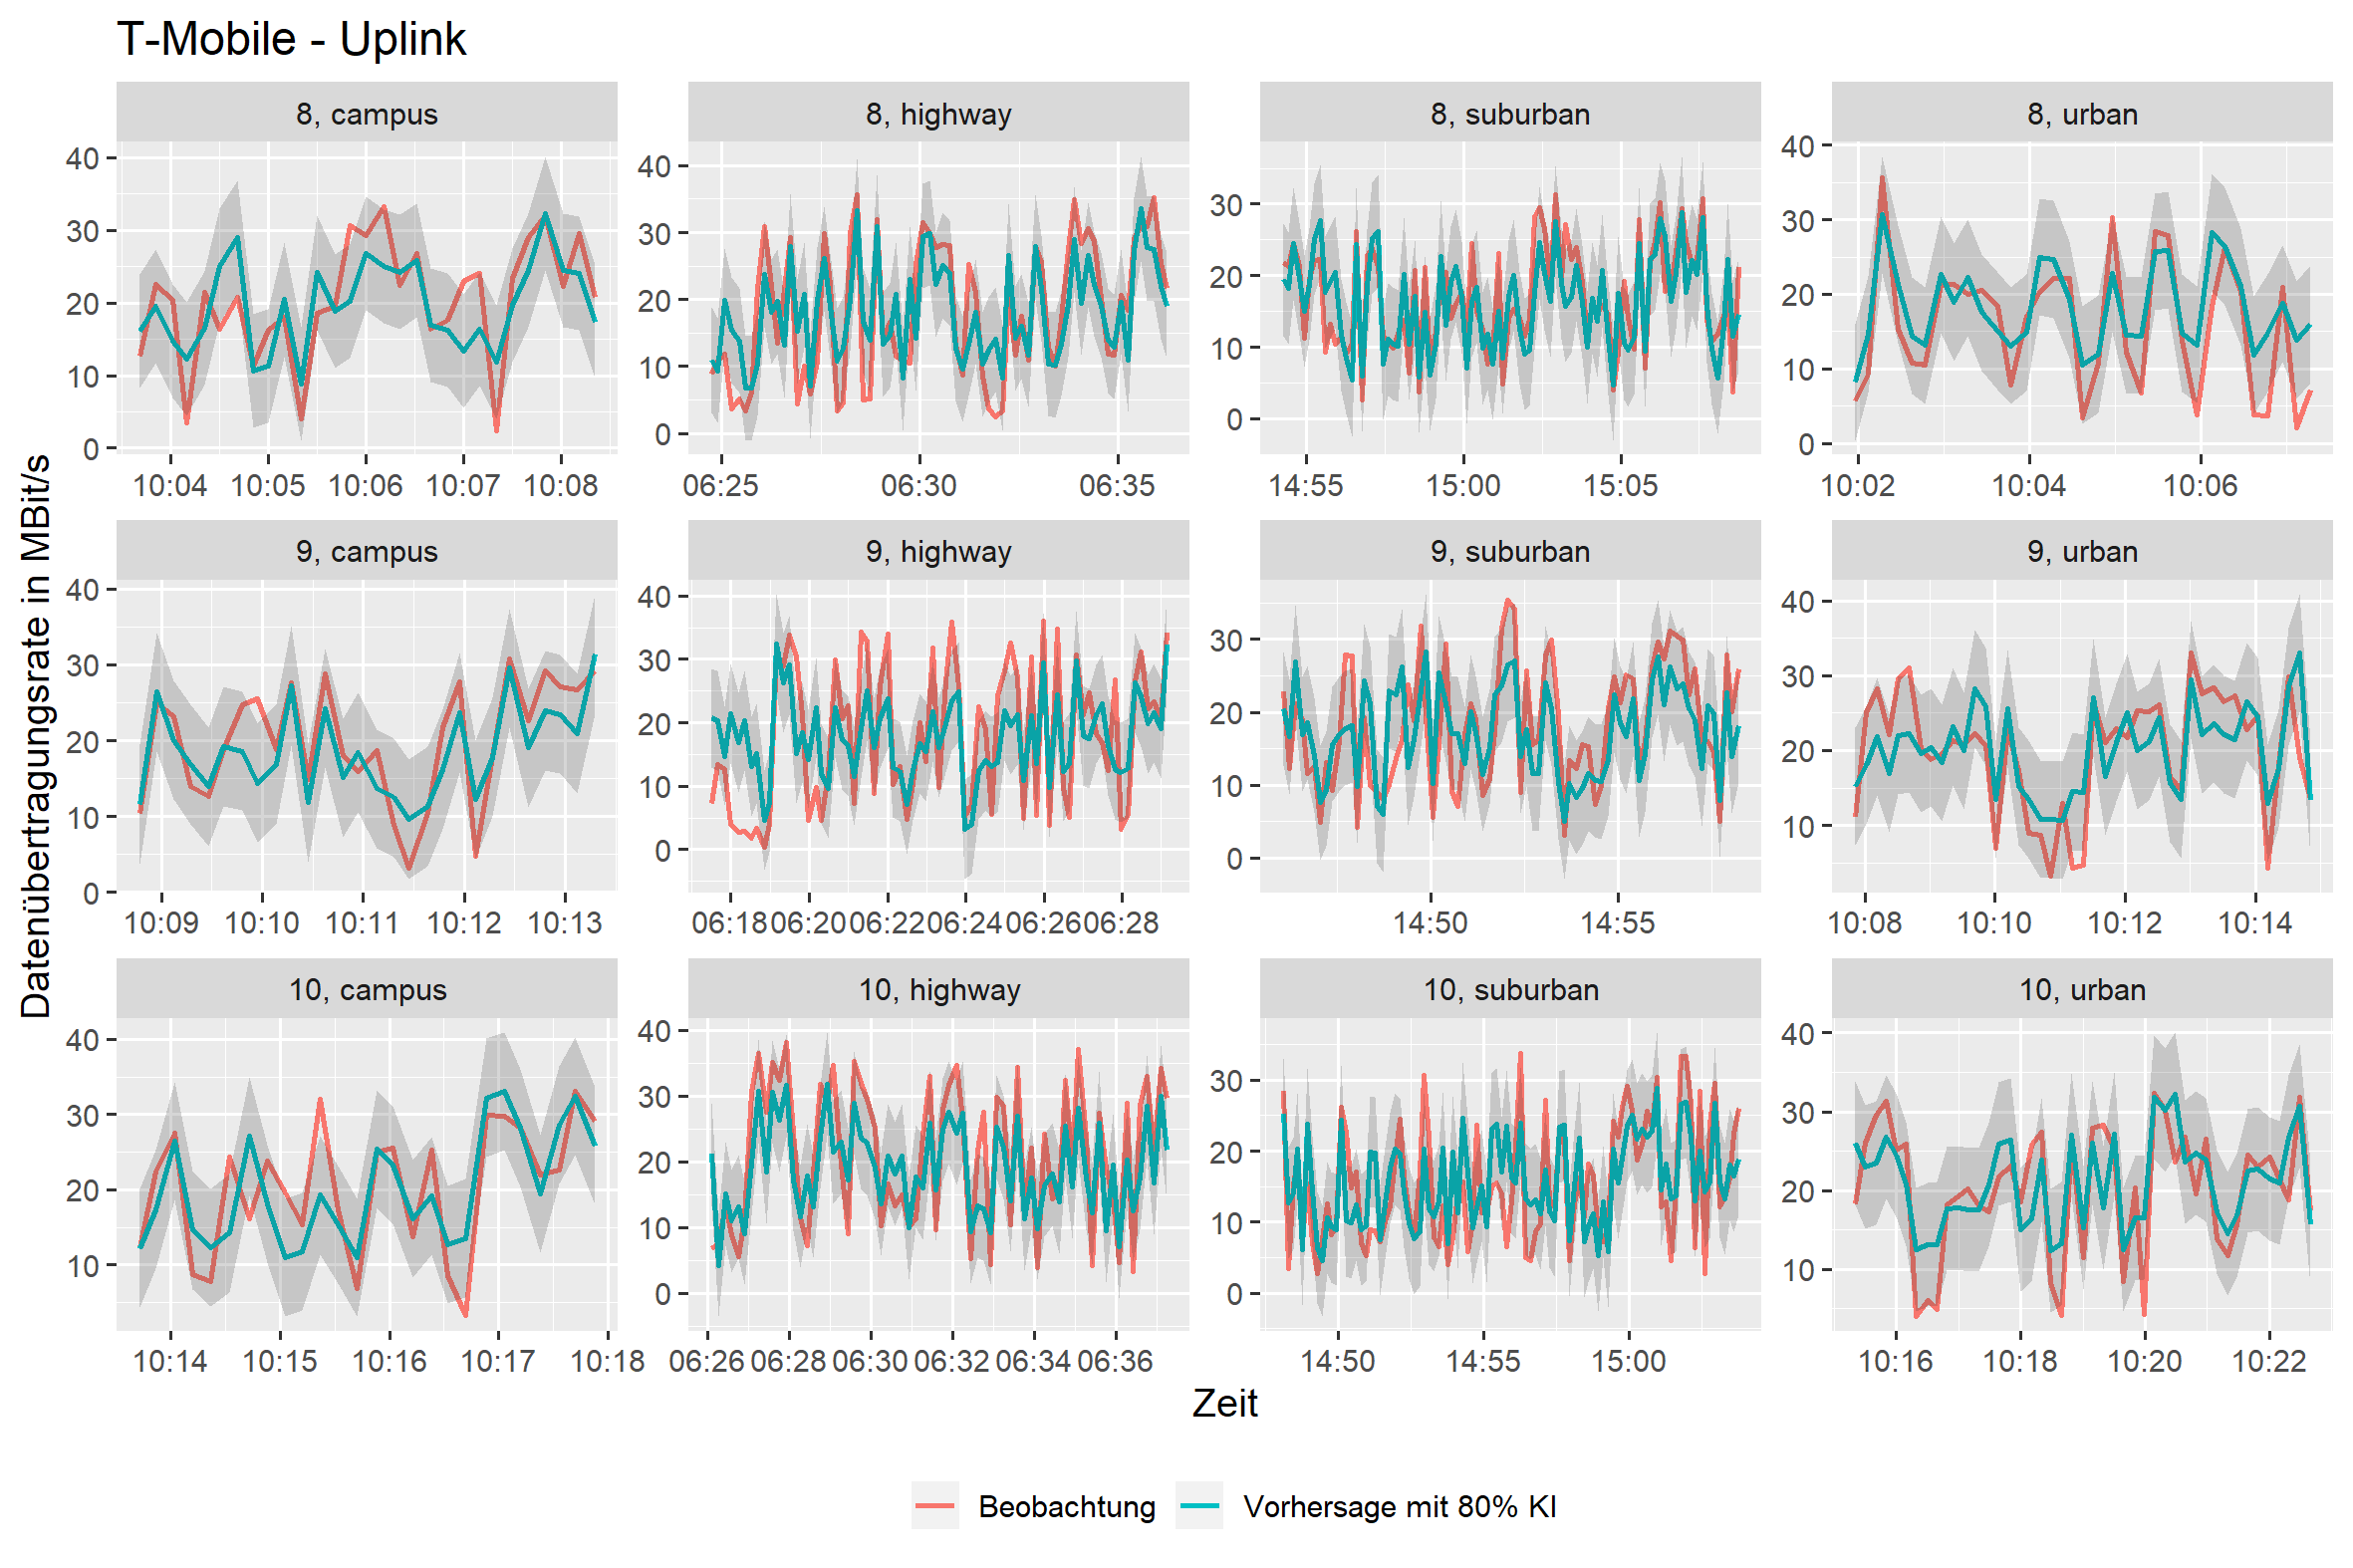
\includegraphics[scale=0.38]{plots/arima/uplink/tmobile_predictions}\\
		\caption{Vorhersage der Datenübertragungsrate des Providers T-Mobile in Richtung Uplink.}
		\label{tmobile_predictions_ul}
	\end{figure}
\end{frame}

\begin{frame}{Regression mit ARMA-Fehlern: Ergebnisse (Uplink)}
	\begin{figure}
		\centering
		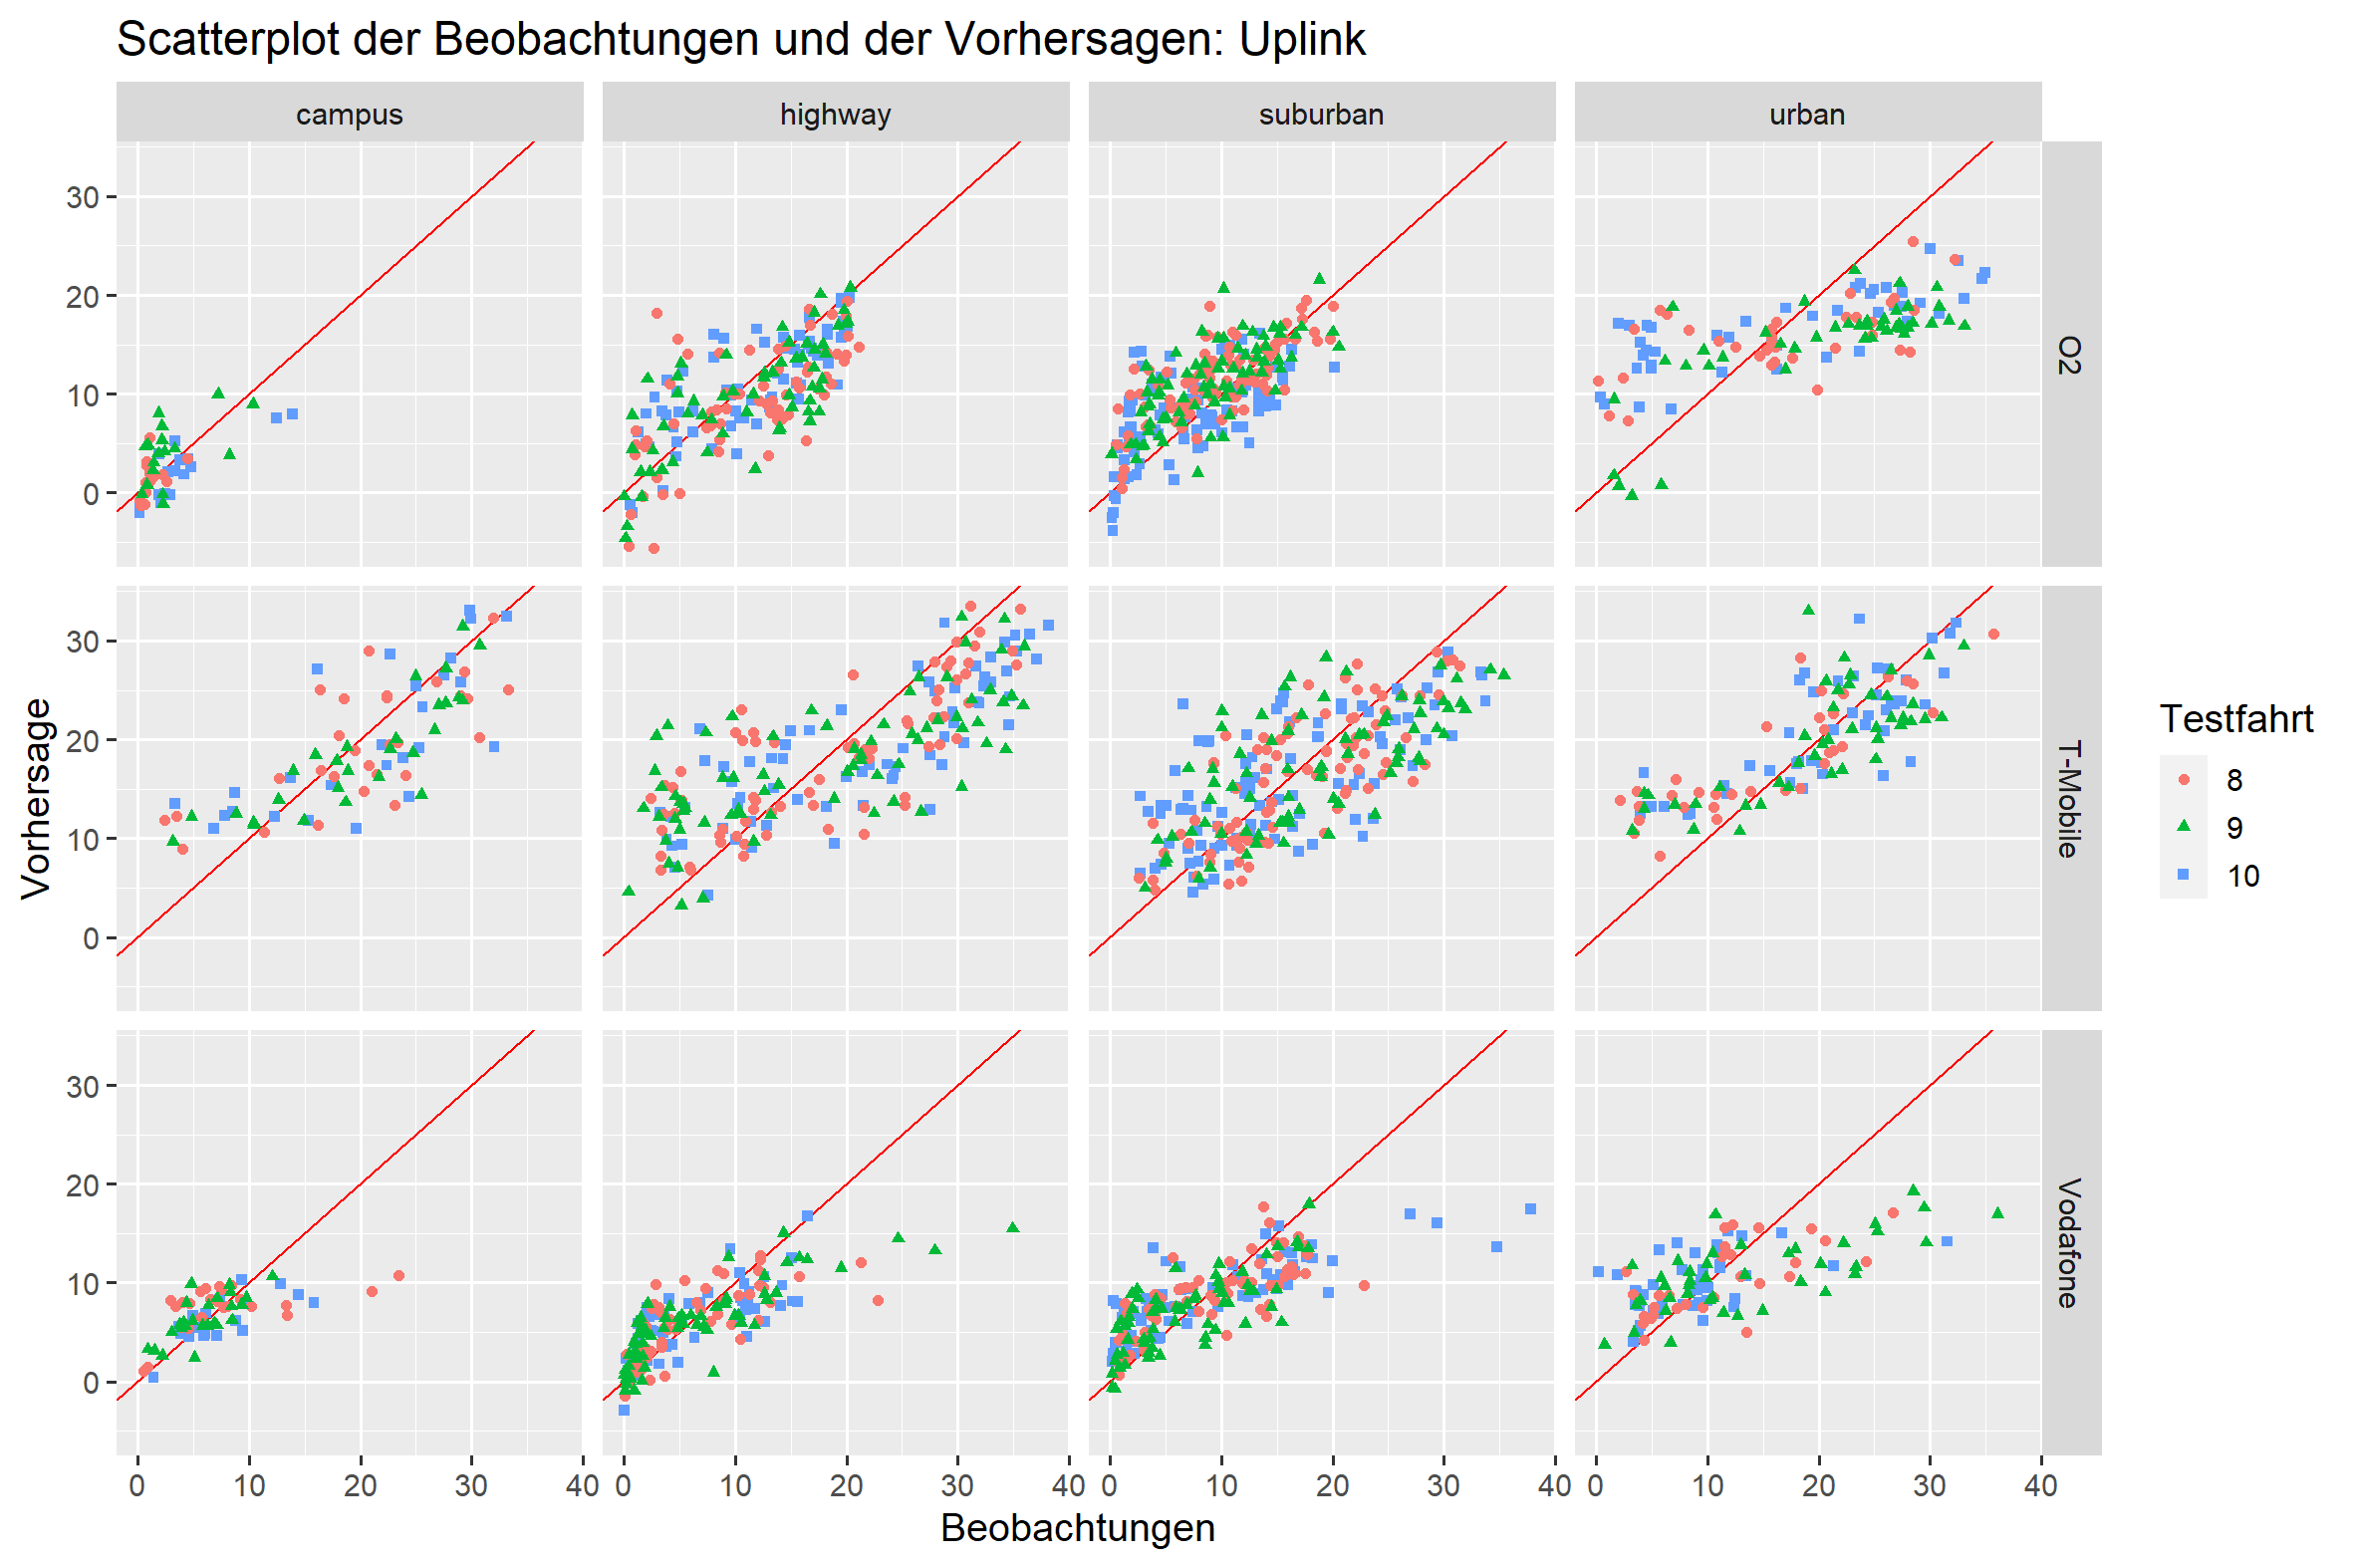
\includegraphics[scale=0.38]{plots/arima/uplink/scatter_colored_axes_fixed}\\
		\caption{Scatterplots der Vorhersagen und Beobachtungen für alle Szenarien und alle Provider in Richtung Uplink.}
		\label{arima_scatter_ul}
	\end{figure}
\end{frame}

\begin{frame}{Regression mit ARMA-Fehlern: Ergebnisse (Downlink)}
	\begin{figure}
		\centering
		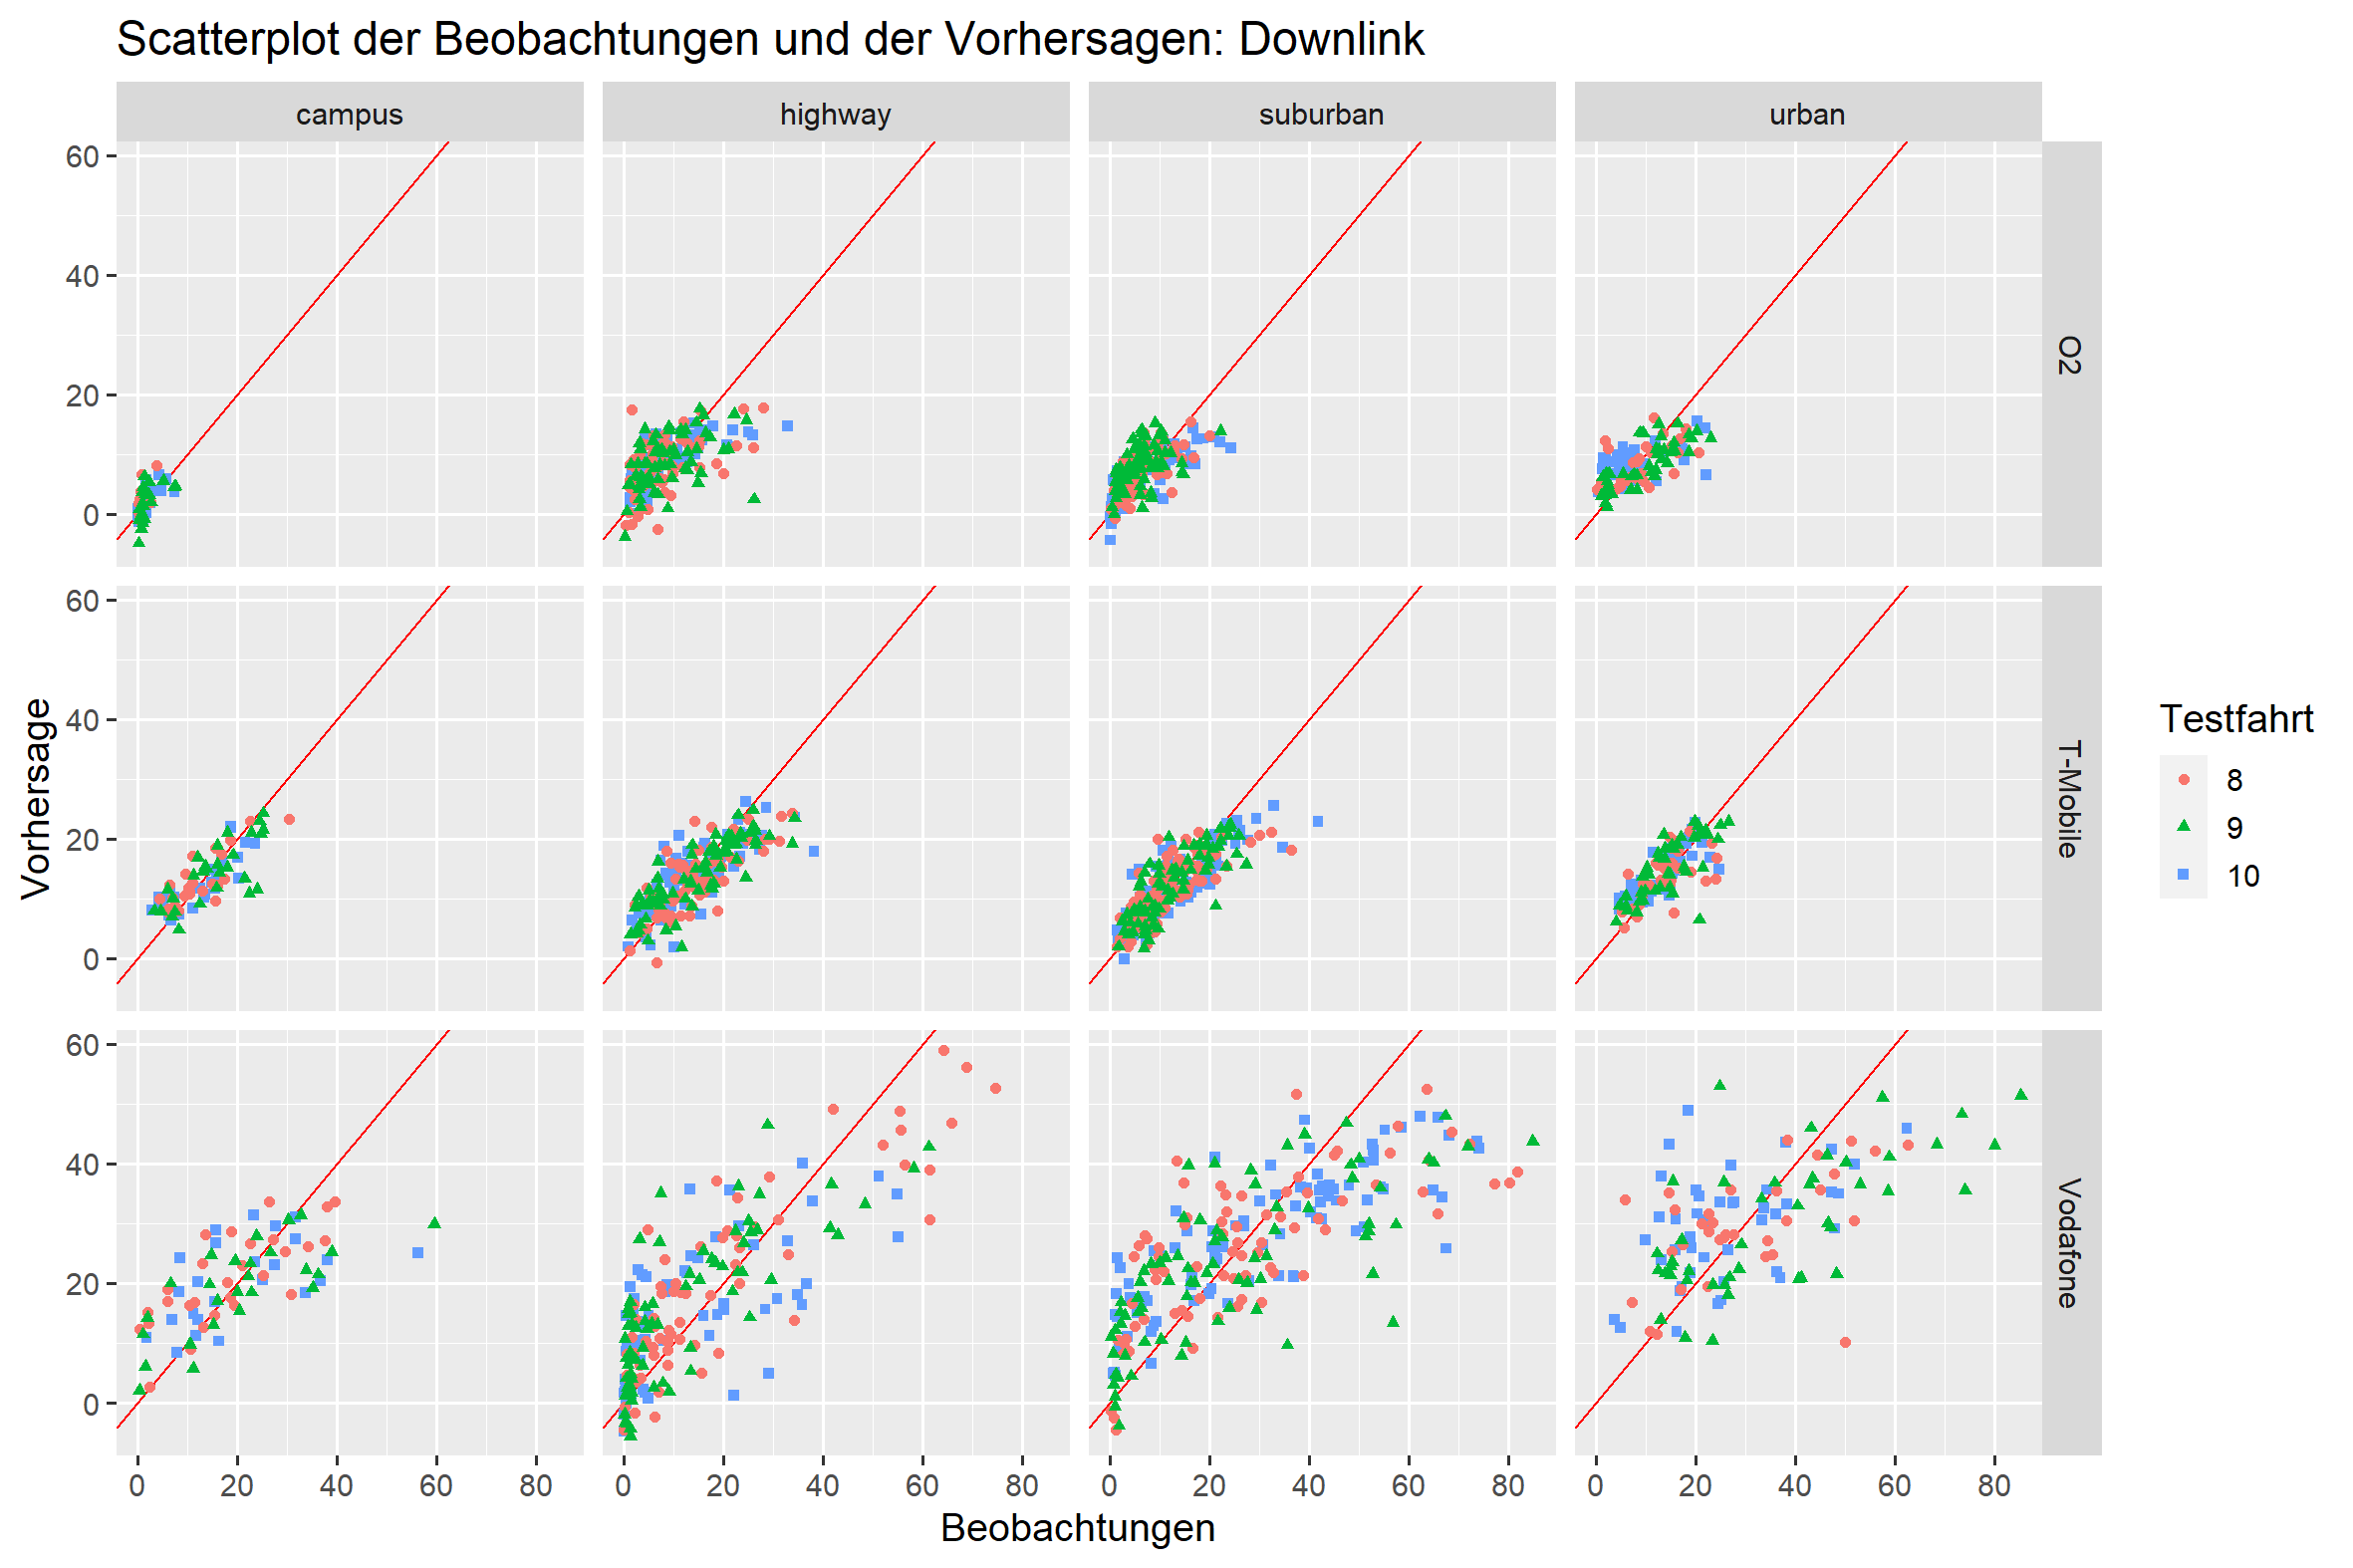
\includegraphics[scale=0.38]{plots/arima/downlink/scatter_colored_axes_fixed}\\
		\caption{Scatterplots der Vorhersagen und Beobachtungen für alle Szenarien und alle Provider in Richtung Downlink.}
		\label{arima_uplink_scatter}
	\end{figure}
\end{frame}




	


